\documentclass[border=10pt,varwidth=20cm]{standalone}
\usepackage{graphicx}
\usepackage{xcolor}

\begin{document}

%{\hspace{0.1cm} \Huge Schematic of approach.}

\bigskip

%\framebox{
\setlength{\fboxrule}{1pt}
%\setlength{\fboxrule}{2pt}
%\fcolorbox{yellow!60!black}{yellow!5!white}
\fcolorbox{black}{white}
{\begin{minipage}[c]{0.985\textwidth}
   \begin{figure}[H]
      \centering
      \vspace{0.3cm}
      {\large \textbf{(a)} Variable selection: Identify relevant parameters and constrain their values.}
      \vspace{0.3cm}
      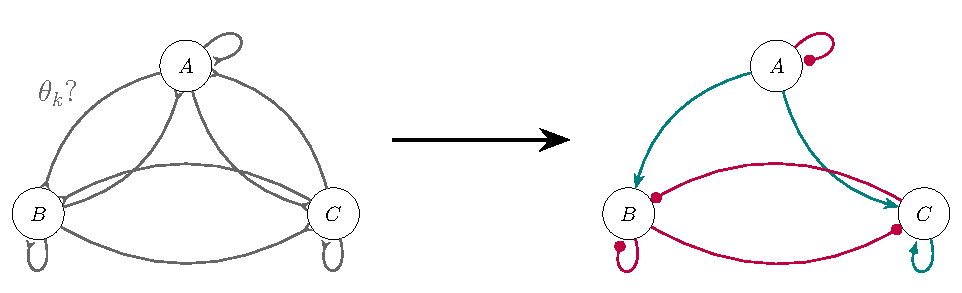
\includegraphics[width=0.5\textwidth]{panel1}
   \end{figure}
\end{minipage}}

\bigskip

\begin{minipage}[c]{0.5\textwidth}
   \begin{figure}[H]
      \vspace{0.3cm}
      {\large \textbf{(b)} The Gibbs sampling algorithm.}
      \vspace{0.3cm}
      \centering      
      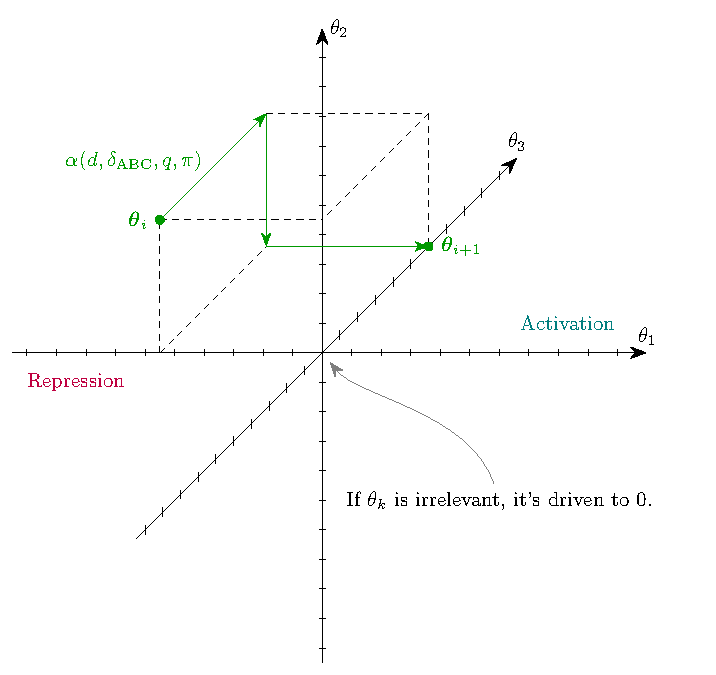
\includegraphics[width=\textwidth]{panel2} 
   \end{figure}
\end{minipage}
%\fcolorbox{violet!80!black}{violet!5!white}
\fcolorbox{black}{white}
{\begin{minipage}[c]{0.48\textwidth}
   \begin{figure}[H]
      \vspace{0.3cm}
      {\large \textbf{(c)} Proposal and prior distributions}
      \vspace{0.3cm}
      \centering
          
      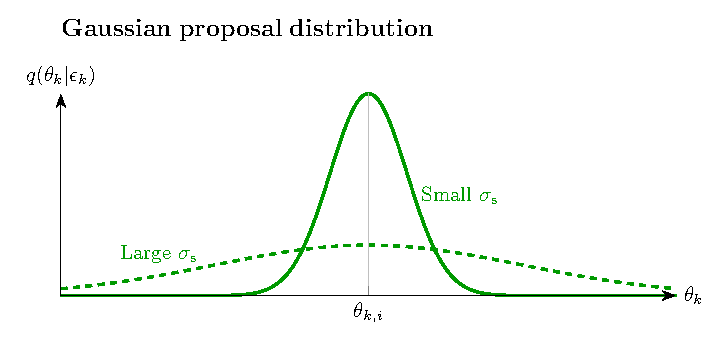
\includegraphics[width=\textwidth]{panel3}
      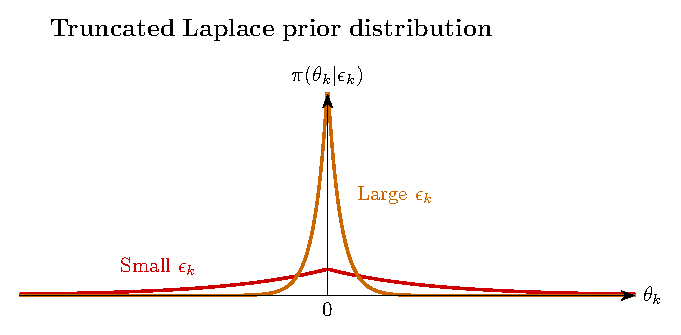
\includegraphics[width=\textwidth]{panel4} 
   \end{figure}
\end{minipage}}

\bigskip

{\begin{minipage}[c]{0.985\textwidth}
   \begin{figure}[H]
      \centering
      \vspace{0.3cm}
      {\large \textbf{(d)} The hyper-parameters are automatically adjusted.}
      \vspace{0.3cm}
      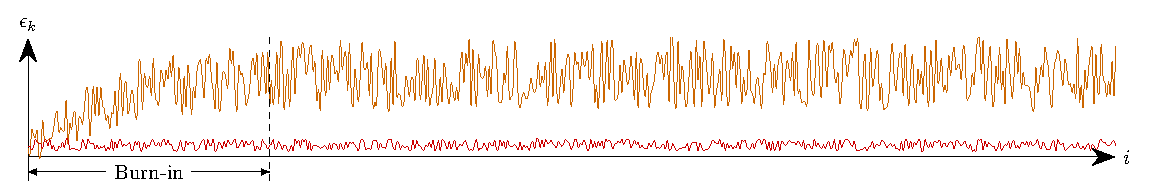
\includegraphics[width=1\textwidth]{panel5}
   \end{figure}
\end{minipage}}

\end{document}